\chapter{Pourquoi la supersymétrie pourrait avoir de l’importance}

\lectureoverview{Les fluctuations du vide relient les sujets de ce chapitre.
Les conditions aux limites produisent la force de Casimir, les effets de boucle menacent la masse du Higgs, de nouvelles particules virtuelles modifient l’évolution des couplages de jauge et l’énergie du vide gouverne l’expansion cosmique. Ces problèmes motivent la supersymétrie à basse énergie, qui pourrait stabiliser l’échelle du Higgs, fournir un candidat à la matière noire et améliorer l’unification des couplages de jauge. Nous construisons ensuite des superchamps à l’aide de coordonnées de Grassmann et utilisons l’intégration de Berezin pour extraire une action supersymétrique.}

\section{Fluctuations du vide entre des plaques réfléchissantes}

Nous revenons à la supersymétrie en commençant par répondre à une question sur l’effet Casimir. Plaçons deux plaques réfléchissantes parallèles séparées par une distance \(d\). Même en l’absence de particules réelles, un champ quantique présente des fluctuations du vide. On peut les représenter comme des processus virtuels ou, de manière équivalente, comme le mouvement de point zéro des modes oscillatoires du champ. Les plaques imposent des conditions aux limites : les fluctuations autorisées entre elles diffèrent donc de celles de l’espace sans restriction.

La grandeur importante n’est pas une valeur absolue de l’énergie zéro, mais la variation produite par un changement de la séparation. Notons \(\mathcal E(d)=E(d)/A\) l’énergie du vide par unité de surface. Dès que \(\mathcal E\) dépend de \(d\), il s’agit d’une énergie potentielle, et la force par unité de surface vaut
\begin{equation}
\frac{F}{A}=-\frac{d\mathcal E}{dd}.
\end{equation}
Ainsi, un réarrangement des processus virtuels devient une force observable. Dans l’exemple électromagnétique classique de plaques parfaitement conductrices, l’énergie et la pression sont
\begin{align}
\mathcal E(d)&=-\frac{\pi^2}{720\,d^3},\\
\frac{F}{A}&=-\frac{\pi^2}{240\,d^4},
\end{align}
dans les unités \(\hbar=c=1\).\editorialnote{Ces coefficients et la distinction entre l’énergie par unité de surface en \(d^{-3}\) et la pression en \(d^{-4}\) répondent à la question de dimension soulevée au tableau. Il s’agit du résultat standard pour des plaques idéales, et non d’une démonstration présentée ici.}Le signe moins indique une attraction.

\begin{classroomqa}
\audiencequestion{La puissance quatrième décrit-elle la force ou l’énergie ? \lecturetimestamp{00:04:39}}
\lecturerresponse{Pour des plaques parallèles dans un espace-temps à quatre dimensions, l’énergie par unité de surface décroît comme \(d^{-3}\), tandis que la dérivation par rapport à \(d\) donne une force par unité de surface qui décroît comme \(d^{-4}\). L’analyse dimensionnelle fixe déjà ces puissances une fois que l’on rétablit \(\hbar\) et \(c\).}
\end{classroomqa}

On résume parfois le calcul en disant que les plaques interrompent les boucles de photons virtuels. Cette représentation est utile à condition de ne pas la prendre trop littéralement. Le calcul précis consiste en une modification du spectre des modes du champ autorisés ou, de manière équivalente, de l’action effective quantique. Ces deux formulations conduisent à la même énergie dépendant de la séparation.

\begin{classroomqa}
\audiencequestion{La force de Casimir peut-elle être répulsive plutôt qu’attractive ? \lecturetimestamp{00:07:48}}
\lecturerresponse{Oui. Le signe n’est pas universel : il dépend des champs, de la géométrie, des matériaux et des conditions aux limites. Les boucles fermioniques ont souvent un signe opposé à celui des boucles bosoniques, ce qui motive la suggestion faite au tableau ; toutefois, la statistique fermionique ne constitue pas à elle seule un théorème général selon lequel toute force de Casimir serait répulsive.\editorialnote{Cette réserve remplace une réponse de cours délibérément hésitante par l’énoncé général nécessaire pour éviter une fausse règle universelle.}}
\end{classroomqa}

\subsection{Qu’est-ce qui constituerait une preuve de l’énergie du vide ?}

La force de Casimir est mesurée, et les observables atomiques sont également sensibles aux boucles du vide. Pourtant, aucun de ces faits ne démontre à lui seul qu’une énergie absolue du vide gravite. Une expérience de Casimir mesure une différence d’énergie due aux conditions aux limites ; on peut décrire la même force sans attribuer de sens opérationnel à une somme de point zéro absolue et non bornée.

Le test décisif vient de la gravité. L’énergie est une charge gravitationnelle. Si le vide porte une densité d’énergie uniforme, celle-ci doit entrer dans les équations d’Einstein et influer sur l’expansion cosmique. L’expansion accélérée de l’Univers constitue donc la preuve gravitationnelle directe d’une composante apparentée au vide.

\begin{classroomqa}
\audiencequestion{Pourquoi les ouvrages de vulgarisation qualifient-ils l’énergie du vide de mystérieuse, comme si les physiciens ne savaient pas ce que c’est ? \lecturetimestamp{00:08:19}}
\lecturerresponse{La théorie quantique des champs attribue une contribution de point zéro à chaque champ ; la possibilité d’une énergie du vide n’a donc rien de mystérieux. Le mystère est quantitatif : pourquoi la valeur gravitationnelle est-elle extraordinairement faible par rapport aux estimations fondées sur les champs quantiques connus et une coupure à haute énergie ? Le fait surprenant est son absence presque totale, et non sa simple existence.}
\end{classroomqa}

Pendant de nombreuses années, la borne supérieure observationnelle était si faible qu’il était psychologiquement tentant de poser la constante cosmologique exactement égale à zéro et de chercher un principe imposant cette annulation. Des observations cosmologiques plus précises ont plutôt révélé une petite valeur non nulle. Cette découverte n’a pas rendu l’énergie du vide étrangère sur le plan conceptuel ; elle a rendu impossible d’ignorer le degré de suppression inexpliqué. La comparaison pertinente dépend de l’échelle ultraviolette supposée, mais toute estimation naturelle à haute énergie exige une annulation considérable.

\section{Action d’une charge supersymétrique sur un état à plusieurs particules}

Avant d’énumérer les raisons de croire à la supersymétrie, dissipons un paradoxe possible. Un nombre arbitrairement grand de bosons peut occuper un même mode, tandis qu’un mode fermionique a un nombre d’occupation égal à zéro ou à un. Si une symétrie échange les bosons et les fermions, transforme-t-elle mille bosons dans un même mode en mille fermions interdits ?

Non. Un générateur fermionique modifie l’état quantique d’un quantum à la fois. Dans le modèle de l’oscillateur, notons \(a\) l’opérateur qui annihile un boson et \(c^\dagger\) celui qui crée son partenaire fermionique. On peut représenter une charge supersymétrique par
\begin{equation}
Q=c^\dagger a.
\end{equation}
Sur un état contenant \(n\) bosons et aucun fermion,
\begin{equation}
Q\ket{n,0}
=\sqrt n\,\ket{n-1,1}.
\end{equation}
Un boson a été supprimé et un fermion a été ajouté. Une nouvelle action de la même charge donne zéro :
\begin{equation}
Q^2=(c^\dagger)^2a^2=0.
\end{equation}
C’est la nilpotence héritée des opérateurs de création fermioniques.

\begin{classroomqa}
\audiencequestion{Si de nombreux bosons occupent le même état, pourquoi une transformation supersymétrique ne produit-elle pas de nombreux fermions dans ce même état, en violation du principe d’exclusion ? \lecturetimestamp{00:12:05}}
\lecturerresponse{Le générateur ne remplace pas toute la population. Il modifie l’état d’une unité de nombre fermionique. On ne peut pas composer la même charge fermionique comme un générateur de rotation ordinaire, car son carré s’annule. Une charge complémentaire peut inverser l’échange, et l’anticommutateur mixte se referme sur la translation temporelle.}
\end{classroomqa}

La dernière phrase est essentielle. L’abréviation \(Q^2=0\) s’applique à une composante chirale individuelle ou à la charge simple que nous venons d’écrire ; elle ne signifie pas que tout produit de charges supersymétriques s’annule. En supersymétrie à quatre dimensions,
\begin{equation}
\{Q_\alpha,\bar Q_{\dot\beta}\}
=2\sigma^\mu_{\alpha\dot\beta}P_\mu,
\end{equation}
alors que
\begin{equation}
\{Q_\alpha,Q_\beta\}=0,
\qquad
\{\bar Q_{\dot\alpha},\bar Q_{\dot\beta}\}=0
\end{equation}
pour l’algèbre minimale sans charges centrales.\editorialnote{Cette forme en composantes précise l’abréviation utilisée en cours : l’action répétée de la même \(Q\) s’annule, tandis qu’une charge supersymétrique et sa conjuguée engendrent une translation.}

\section{Trois raisons de rechercher la supersymétrie à basse énergie}

\begin{classroomqa}
\audiencequestion{Existe-t-il d’autres motivations pour la supersymétrie que l’annulation de l’énergie du vide ? \lecturetimestamp{00:15:06}}
\lecturerresponse{Trois motivations étroitement liées se dégagent : le contrôle de l’auto-énergie du Higgs, un éventuel candidat stable à la matière noire et une convergence beaucoup plus précise des couplages de jauge à haute énergie. Aucune ne prouve que la supersymétrie se réalise dans la nature, mais ensemble, elles en font une théorie sérieuse à mettre à l’épreuve.}
\end{classroomqa}

L’expression \emph{supersymétrie à basse énergie} est relative. Elle ne signifie pas que les partenaires supersymétriques sont légers à l’échelle quotidienne ; elle signifie que leurs masses ne sont pas très supérieures aux échelles électrofaible et des accélérateurs. Les trois arguments s’affaiblissent si les masses des partenaires supersymétriques sont poussées arbitrairement haut.

\subsection{Protéger l’échelle du Higgs}

La masse d’un scalaire est exceptionnellement sensible à la physique des hautes énergies. Schématiquement, une boucle bosonique produit une correction de la forme
\begin{equation}
\delta m_H^2\big|_{\mathrm B}
\sim +\frac{\lambda}{16\pi^2}\Lambda^2,
\end{equation}
où \(\Lambda\) désigne l’échelle jusqu’à laquelle on utilise la théorie effective. Une boucle fermionique porte le signe opposé,
\begin{equation}
\delta m_H^2\big|_{\mathrm F}
\sim -\frac{|y|^2}{8\pi^2}\Lambda^2.
\end{equation}
Les coefficients dépendent de l’interaction et des multiplicités des champs, mais la supersymétrie établit entre eux des relations qui annulent la sensibilité ultraviolette dominante entre partenaires.\editorialnote{Ces formules schématiques de boucle exposent le fondement mathématique de l’argument qualitatif sur l’auto-énergie. Elles ne sont pas destinées à constituer un calcul complet de la masse du Higgs du Modèle standard.}

Cela importe, car la valeur moyenne du champ de Higgs fixe l’échelle électrofaible. Les masses des bosons de jauge et des fermions vérifient des relations telles que
\begin{equation}
m_W=\frac{gv}{2},
\qquad
m_f=\frac{y_fv}{\sqrt2}.
\end{equation}
Si le secteur de Higgs était naturellement entraîné vers une échelle immense, le spectre familier des particules à basse énergie disparaîtrait, à moins d’ajuster les paramètres nus avec une précision extrême pour compenser les corrections radiatives.

Une supersymétrie exacte rendrait l’annulation exacte, mais la supersymétrie exacte est déjà exclue par les masses inégales des bosons et fermions observés. Avec une supersymétrie brisée doucement, la sensibilité quadratique est remplacée par une dépendance aux écarts de masse entre partenaires, schématiquement
\begin{equation}
\delta m_H^2
\sim
\frac{g^2}{16\pi^2}
\left(m_{\mathrm{soft}}^2-m_{\mathrm{ordinary}}^2\right)
\ln\frac{\Lambda^2}{m_{\mathrm{soft}}^2}.
\end{equation}
L’annulation ne reste utile que si l’écart n’est pas trop grand.

\subsection{Un état final stable pour les cascades de désintégration de la matière noire}

Séparons le spectre en particules ordinaires et en leurs partenaires supersymétriques. Un fermion a un partenaire bosonique ; un boson a un partenaire fermionique. Si les interactions conservent une parité qui distingue ces deux classes, toute désintégration d’un partenaire supersymétrique doit en laisser un autre :
\begin{equation}
\widetilde X
\longrightarrow X+\widetilde Y
\longrightarrow X+Y+\widetilde Z
\longrightarrow\cdots.
\end{equation}
La cascade ne peut pas éliminer son dernier partenaire supersymétrique. Elle se termine donc par la particule supersymétrique la plus légère, le LSP.

La symétrie couramment utilisée est la parité \(R\),
\begin{equation}
R_p=(-1)^{3(B-L)+2s}.
\end{equation}
Les particules du Modèle standard ont \(R_p=+1\), tandis que leurs partenaires supersymétriques ont \(R_p=-1\). Si \(R_p\) est exacte, chaque interaction comporte un nombre pair de partenaires supersymétriques et le LSP est stable.\editorialnote{La supersymétrie seule ne garantit pas la stabilité du LSP. Cette stabilité exige la conservation de la parité \(R\) ou d’une autre symétrie ayant la même conséquence ; sans elle, le LSP peut se désintégrer.}

La matière noire doit survivre au moins pendant des durées cosmologiques. Elle doit aussi interagir assez faiblement pour traverser à plusieurs reprises le disque galactique visible sans perdre une quantité importante d’énergie. Une population chargée électriquement ou soumise à l’interaction forte diffuserait, dissiperait de l’énergie et tendrait à s’effondrer vers la même structure mince que la matière ordinaire. Le halo étendu observé indique plutôt une composante neutre et faiblement interactive.

Cela ne permet pas d’identifier le LSP de façon unique. Selon le modèle et le schéma de brisure de symétrie, le candidat pourrait être un mélange neutre de jauginos électrofaibles et de higgsinos, ou bien un gravitino. Les candidats chargés ou colorés sont soumis à de fortes contraintes. La supersymétrie ne fournit pas une réponse garantie, mais un mécanisme naturel qui produit un état final neutre et à longue durée de vie.

\section{Couplages qui évoluent et indice d’unification}

La troisième motivation part de l’écrantage des charges. La valeur mesurée d’un couplage dépend de l’échelle d’énergie, car des particules virtuelles habillent l’interaction. En électromagnétisme, une boucle électron-positron insérée dans un propagateur de photon écrante la charge à grande distance. À plus courte distance, ou pour un transfert d’impulsion plus élevé, une moindre partie de ce nuage de polarisation se trouve entre les sondes ; la charge effective est donc plus grande.

Posons
\begin{equation}
\alpha_i=\frac{g_i^2}{4\pi}.
\end{equation}
À une boucle, l’inverse du couplage évolue linéairement avec le logarithme de l’énergie :
\begin{equation}
\frac{d\alpha_i^{-1}}{d\ln\mu}
=-\frac{b_i}{2\pi}.
\end{equation}
Ainsi,
\begin{equation}
\alpha_i^{-1}(\mu)
=\alpha_i^{-1}(\mu_0)
-\frac{b_i}{2\pi}\ln\frac{\mu}{\mu_0}.
\end{equation}
\editorialnote{Cette équation à une boucle donne la formulation précise des droites presque rectilignes tracées en fonction du logarithme de l’énergie. Les seuils et les corrections d’ordre supérieur courbent légèrement ces droites.}

Au-dessus de l’échelle électrofaible, les trois couplages de jauge fondamentaux sont ceux de
\begin{equation}
U(1)_Y,\qquad SU(2)_L,\qquad SU(3)_c.
\end{equation}
Le couplage électromagnétique utilisé comme repère à basse énergie est une combinaison des deux premiers après la brisure de la symétrie électrofaible. Pour la QCD, les champs de jauge non abéliens produisent un anti-écrantage : le couplage fort diminue à courte distance, phénomène appelé liberté asymptotique. Par conséquent, \(\alpha_3^{-1}\) augmente avec \(\ln\mu\), tandis que les inverses des autres couplages ont des pentes différentes.

Les courbes du Modèle standard semblent se rapprocher, mais elles ne se rencontrent pas en un même point. Les partenaires supersymétriques modifient les boucles virtuelles et donc les coefficients \(b_i\). Avec la normalisation conventionnelle de grande unification,
\begin{align}
(b_1,b_2,b_3)_{\mathrm{SM}}
&=\left(\frac{41}{10},-\frac{19}{6},-7\right),\\
(b_1,b_2,b_3)_{\mathrm{MSSM}}
&=\left(\frac{33}{5},1,-3\right).
\end{align}
les courbes extrapolées de la théorie supersymétrique se rencontrent avec une bien meilleure précision, près de
\begin{equation}
M_{\mathrm{GUT}}\sim 10^{16}\ \mathrm{GeV}.
\end{equation}
Aucune expérience n’atteint directement cette échelle. On mesure les couplages à basse énergie, le contenu en champs détermine leur évolution, puis on extrapole les courbes sur de nombreux ordres de grandeur. Deux droites se croisent toujours quelque part ; le fait non trivial est que trois droites indépendantes se rencontrent à proximité d’un même point.

\begin{classroomqa}
\audiencequestion{L’extrapolation améliorée suppose-t-elle une supersymétrie exacte et des masses identiques pour les partenaires ? \lecturetimestamp{00:38:09}}
\lecturerresponse{Non. La supersymétrie est brisée, et les masses sont donc différentes. Ce qui importe, c’est le moment où les boucles des partenaires supersymétriques entrent en jeu dans l’évolution. Si les partenaires ne sont pas trop lourds, les pentes changent assez tôt pour que les trois couplages convergent. S’ils sont extrêmement lourds, les seuils supersymétriques apparaissent trop tard et la convergence améliorée disparaît.}
\end{classroomqa}

Les corrections de seuil et le spectre inconnu à haute énergie empêchent d’affirmer littéralement que les trois droites se rencontrent avec une exactitude mathématique. Le résultat reste néanmoins frappant : la même échelle approximative des partenaires supersymétriques qui aide à stabiliser le Higgs et fournit un candidat thermique à la matière noire améliore aussi l’unification.

\subsection{Gravité et échelle commune de haute énergie}

La gravité se comporte différemment, car sa charge est l’énergie elle-même. Une mesure sans dimension utile à l’énergie du centre de masse \(E\) est
\begin{equation}
\alpha_G(E)\sim GE^2
=\left(\frac{E}{M_{\mathrm{Pl}}}\right)^2.
\end{equation}
Aux énergies ordinaires, cette quantité est extraordinairement petite, mais elle croît comme le carré de \(E\). Son inverse diminue donc bien plus rapidement que les inverses des couplages de jauge, qui évoluent de façon logarithmique, et devient de l’ordre de l’unité près de l’échelle de Planck.

Cette comparaison suggère que toutes les interactions pourraient être gouvernées par des échelles élevées voisines, mais elle est moins nette que l’unification des couplages de jauge. Les couplages de jauge sont des paramètres sans dimension dans les théories des champs renormalisables ; la constante de Newton a une dimension, si bien que représenter la gravité sur le même graphique exige une convention.

\begin{classroomqa}
\audiencequestion{Les partenaires supersymétriques participent-ils aux trois mêmes interactions de jauge ou définissent-ils de nouvelles forces ? \lecturetimestamp{00:42:35}}
\lecturerresponse{Ils portent les mêmes nombres quantiques de jauge que leurs partenaires. Un sélectron a la charge électrique de l’électron, et un squark possède les charges de couleur et électrofaibles correspondantes à celles du quark, même si leurs spins et leurs masses diffèrent. Leurs boucles modifient donc les mêmes interactions de jauge au lieu d’en introduire trois nouvelles.}
\end{classroomqa}

\begin{classroomqa}
\audiencequestion{La découverte d’un partenaire supersymétrique au LHC constituerait-elle une preuve définitive de la supersymétrie ? \lecturetimestamp{00:43:27}}
\lecturerresponse{Une particule inhabituelle ne suffirait pas à elle seule, quel que soit le nom qu’on lui donne ; en revanche, un spectre de partenaires supersymétriques qui respecterait les relations de supersymétrie entre spins, charges, masses et couplages serait très caractéristique. La supersymétrie impose de nombreuses contraintes corrélées : le schéma détaillé des interactions constituerait donc le test décisif.}
\end{classroomqa}

\subsection{Pourquoi déplacer l’échelle a un coût}

Si les partenaires supersymétriques se trouvent juste au-delà des limites expérimentales, les trois motivations peuvent encore s’appliquer. Si leurs masses augmentent de plusieurs ordres de grandeur, chacun des arguments s’affaiblit :
\begin{enumerate}
\item Les annulations de la masse du Higgs laissent une forte sensibilité résiduelle à l’écart de masse.
\item Un reliquat thermique conventionnel à l’échelle électrofaible n’apparaît plus à l’échelle attendue.
\item Les seuils liés à l’évolution des couplages se déplacent vers les hautes énergies, et les trois couplages se rencontrent avec moins de précision.
\end{enumerate}
La supersymétrie pourrait toujours exister à une échelle beaucoup plus élevée, mais elle ne résoudrait plus ces problèmes particuliers de basse énergie avec la même économie. La longévité de cette idée ne prouve pas que la nature doit l’adopter ; elle montre que la proposition est suffisamment cohérente pour mériter un test décisif.

\section{Ce que la cosmologie peut et ne peut pas nous apprendre sur la matière noire}

\begin{classroomqa}
\audiencequestion{La cosmologie standard peut-elle déterminer la quantité de matière noire et la masse de chaque particule de matière noire, comme la nucléosynthèse impose des contraintes sur l’hydrogène et l’hélium ? \lecturetimestamp{00:46:32}}
\lecturerresponse{La cosmologie mesure très bien la densité totale de masse de matière noire, mais cette densité ne permet pas à elle seule de distinguer la masse du nombre de particules. Une même densité peut être portée par quelques particules lourdes ou par un nombre immense de particules très légères. Il faut une théorie supplémentaire ou des observations non gravitationnelles pour identifier la particule microscopique.}
\end{classroomqa}

Deux grandes possibilités illustrent cette ambiguïté. Une particule faiblement interactive, proche de l’échelle électrofaible ou du TeV, peut se découpler du bain thermique chaud. À l’autre extrême, un boson extrêmement léger comme l’axion peut occuper une configuration cohérente de champ ou un condensat. Le fait que les deux mécanismes les mieux développés se situent près des extrêmes opposés n’interdit pas les possibilités intermédiaires.

La structure du halo impose elle-même une contrainte importante. La matière noire traverse la matière ordinaire avec peu de frottement et reste donc étendue dans l’espace au lieu de s’effondrer en un disque lumineux. Les courbes de rotation et d’autres phénomènes gravitationnels nous indiquent que cette masse est présente, mais ne permettent pas à eux seuls de dénombrer les particules.

\begin{classroomqa}
\audiencequestion{L’Univers primordial aurait-il pu ne contenir au départ que des superparticules, qui se seraient ensuite désintégrées en particules que nous observons ? \lecturetimestamp{00:49:11}}
\lecturerresponse{À des températures très supérieures à toutes les masses pertinentes, les réactions rapides conduisent les espèces vers l’équilibre thermique plutôt que vers une population initiale arbitraire constituée d’une seule sorte de particules. Les collisions ordinaires créent des partenaires supersymétriques lorsqu’ils sont sous-abondants, tandis que les collisions et désintégrations de partenaires supersymétriques réalimentent la population de particules ordinaires. L’abondance précise dépend des interactions et des degrés de liberté, mais le plasma chaud tend continuellement vers l’équilibre.}
\end{classroomqa}

À mesure que l’Univers se refroidit, les espèces massives voient leur abondance supprimée par le facteur de Boltzmann et s’annihilent ou se désintègrent. Un LSP stable cesse de suivre l’équilibre lorsque son taux d’interaction devient inférieur au taux d’expansion cosmique :
\begin{equation}
\Gamma_{\mathrm{ann}}
\sim n\langle\sigma v\rangle
\lesssim H.
\end{equation}
Les particules restantes constituent une abondance relique.\editorialnote{Ce critère de découplage donne la formulation quantitative standard qui complète l’argument de l’équilibre thermique. D’autres candidats au rôle de LSP, notamment les gravitinos à couplage très faible, peuvent avoir une histoire non thermique.}

\begin{classroomqa}
\audiencequestion{De quelle particule ordinaire le LSP est-il le partenaire, et doit-il être non interactif ? \lecturetimestamp{00:51:05}}
\lecturerresponse{Il n’existe pas de réponse indépendante du modèle. On s’attend à ce qu’un LSP viable comme matière noire soit électriquement neutre et incolore, mais il n’a pas besoin d’être complètement non interactif. Il peut être un mélange apparenté au photon, aux bosons de jauge faibles et aux champs de Higgs, ou bien être le gravitino. Son identité précise découle du spectre de brisure de la supersymétrie.}
\end{classroomqa}

\section{Diagrammes du vide, diagrammes d’auto-énergie et expansion}

\begin{classroomqa}
\audiencequestion{Quelle différence y a-t-il entre la divergence du Higgs et celle de l’énergie du vide ? \lecturetimestamp{00:52:09}}
\lecturerresponse{Un diagramme du vide ne comporte aucune ligne de particule externe ; il modifie l’action effective du vide et contribue à son énergie. Un diagramme d’auto-énergie du Higgs comporte deux jambes externes de Higgs ; il modifie le propagateur du Higgs et donc sa masse. Les deux mettent en jeu des fluctuations virtuelles, mais répondent à des questions différentes.}
\end{classroomqa}

On peut se représenter une particule réelle comme une impureté insérée dans le vide. Les fluctuations du vide qui se couplent à cette impureté modifient sa propagation et sa masse. Les plaques de Casimir modifient elles aussi les fluctuations du vide, mais par l’intermédiaire de conditions aux limites macroscopiques. Dans les deux cas, les fluctuations quantiques réagissent à ce qui a été introduit ; c’est l’observable corrigée qui diffère.

\vspace{-2pt}\subsection{La matière, le rayonnement et l’énergie du vide se diluent différemment}

Soit \(a(t)\) le facteur d’échelle cosmologique, et
\begin{equation}
H=\frac{\dot a}{a}
\end{equation}
le paramètre de Hubble. La conservation locale du tenseur énergie-impulsion dans un Univers homogène donne
\begin{equation}
\dot\rho+3H(\rho+p)=0.
\end{equation}
Pour une équation d’état \(p=w\rho\), on obtient par intégration
\begin{equation}
\rho(a)\propto a^{-3(1+w)}.
\end{equation}
\editorialnote{L’équation de continuité fournit la dérivation concise qui sous-tend les explications fondées sur le dénombrement des particules et l’étirement des longueurs d’onde.}

Pour la matière froide non relativiste, \(p\approx0\), donc
\begin{equation}
\rho_m\propto a^{-3}.
\end{equation}
Un volume comobile fixé croît comme \(a^3\), tandis que l’énergie de masse de ses particules reste approximativement constante.

Pour le rayonnement, \(p=\rho/3\), et
\begin{equation}
\rho_r\propto a^{-4}.
\end{equation}
Trois puissances proviennent de la dilution de la densité numérique. La quatrième est due au décalage vers le rouge :
\begin{equation}
\lambda\propto a,
\qquad
E_\gamma=\frac{2\pi\hbar c}{\lambda}\propto a^{-1}.
\end{equation}

\begin{classroomqa}
\audiencequestion{Si le photon possède une fonction d’onde, pourquoi peut-on le considérer comme une particule plutôt que comme une onde pour dériver la loi de dilution ? \lecturetimestamp{00:58:21}}
\lecturerresponse{Cette distinction ne change pas la loi d’échelle. Dans la description en termes de particules, le nombre de quanta dans un volume comobile est fixé et l’énergie de chaque quantum subit un décalage vers le rouge en \(a^{-1}\). Dans la description classique en termes d’ondes, la longueur d’onde s’étire et l’énergie du champ diminue de la même quantité. On peut employer la formulation qui rend l’expansion la plus facile à comprendre.}
\end{classroomqa}

L’énergie du vide vérifie \(p_\Lambda=-\rho_\Lambda\), donc
\begin{equation}
\rho_\Lambda=\text{constant}.
\end{equation}
Elle ne se dilue pas lorsque l’espace se dilate. En effet, une région comobile contient
\begin{equation}
E_\Lambda=\rho_\Lambda a^3V_0,
\end{equation}
ce qui augmente avec son volume physique. C’est ce fait qui soulève la question de la conservation de l’énergie, que nous aborderons bientôt.

Ces différentes puissances structurent l’histoire cosmique. Le rayonnement décroît le plus vite, la matière décroît plus lentement, et l’énergie du vide ne décroît pas du tout. Une faible contribution du vide peut donc être négligeable dans l’Univers primordial et dominer à une époque tardive. Selon les valeurs approximatives évoquées ici, le budget énergétique actuel comprend environ \(70\%\) d’énergie du vide et \(30\%\) de matière, le rayonnement étant bien moindre.

\section{La géométrie égale l’énergie}

La composante temporelle-temporelle des équations d’Einstein transforme les lois d’échelle précédentes en dynamique. Le tableau commence par un slogan et un seul terme géométrique.

\begin{figure}[H]\centering
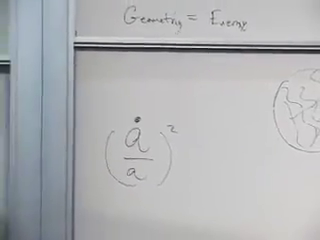
\includegraphics[width=0.68\textwidth]{lecture_06_figure_03.png}\lectureframe{01:06:37.088}\caption{\emph{La géométrie égale l’énergie}, avec le terme d’expansion \(H^2=(\dot a/a)^2\) inscrit en dessous.}\end{figure}

Pour un Univers homogène et isotrope, la première équation de Friedmann est
\begin{equation}
H^2+\frac{k}{a^2}
=\frac{8\pi G}{3}\rho,
\end{equation}
dans les unités \(c=1\), où \(k=+1,0,-1\) désigne une géométrie spatiale fermée, plate ou ouverte, et
\begin{equation}
\rho
=\rho_{\mathrm{ordinary}}
+\rho_{\mathrm{dark}}
+\rho_{\mathrm{radiation}}
+\rho_{\mathrm{vacuum}}.
\end{equation}
Le signe apparaissant à côté de \(1/a^2\) dépend du fait que le terme de courbure soit laissé à gauche ou déplacé à droite, ainsi que de la valeur de \(k\).

\begin{figure}[H]\centering
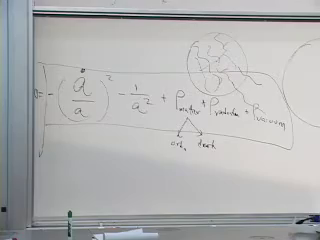
\includegraphics[width=0.96\textwidth]{lecture_06_figure_04.png}\lectureframe{01:08:46.794}\caption{Le bilan complet au tableau : l’expansion et la courbure spatiale du côté géométrique, la matière, le rayonnement et l’énergie du vide du côté des sources. La matière est en outre séparée en composantes ordinaire et noire.}\end{figure}

\subsection{La contrainte hamiltonienne cosmologique}

\begin{classroomqa}
\audiencequestion{Si l’énergie du vide dans une région comobile augmente avec l’expansion de l’Univers, existe-t-il une densité d’énergie nette constante ou une énergie totale conservée ? \lecturetimestamp{01:01:51}}
\lecturerresponse{La relativité générale ne fournit pas d’énergie globale universelle pour un espace-temps en expansion arbitraire. Toutefois, dans la réduction cosmologique homogène, l’équation d’Einstein temporelle-temporelle est une contrainte hamiltonienne. Lorsque la géométrie et la matière sont placées du même côté, le hamiltonien soumis à cette contrainte s’annule. Les termes de matière qui varient sont compensés par les degrés de liberté gravitationnels, plutôt que par une énergie ordinaire fixe dans une boîte.}
\end{classroomqa}

Schématiquement, l’énoncé canonique est
\begin{equation}
\mathcal H_{\mathrm{gravity}}
+\mathcal H_{\mathrm{matter}}
=0.
\end{equation}
C’est là le sens précis de l’affirmation selon laquelle l’énergie totale est nulle. Il s’agit d’une équation du mouvement imposée par l’invariance par reparamétrisation du temps, et non de l’affirmation que chaque densité d’énergie locale s’annule. Dans un volume comobile, l’énergie de la matière ordinaire reste à peu près constante, celle du rayonnement diminue et l’énergie du vide augmente ; dans le même temps, la contribution gravitationnelle et le taux d’expansion s’ajustent de sorte que la contrainte d’Einstein reste satisfaite.

La conservation locale reste exacte :
\begin{equation}
\nabla_\mu T^{\mu\nu}=0.
\end{equation}
Pour le fluide homogène, il s’agit précisément de l’équation de continuité
\(\dot\rho+3H(\rho+p)=0\). Ce qui échoue en général, c’est l’intuition issue de l’espace-temps plat selon laquelle il devrait aussi exister une somme globale de l’énergie de la matière, indépendante des coordonnées et conservée dans un univers en expansion.\editorialnote{Cette distinction précise l’affirmation pédagogique selon laquelle l’énergie est toujours nulle : la conservation covariante locale et la contrainte hamiltonienne cosmologique sont exactes, tandis qu’une énergie globale unique de la matière et de la gravitation n’est généralement pas définie.}

\begin{classroomqa}\audiencequestion{La contrainte nulle est-elle la condition qui détermine si l’Univers est ouvert, fermé ou plat ? \lecturetimestamp{01:04:42}}\lecturerresponse{Non. La contrainte hamiltonienne s’applique dans tous les cas. Les univers ouvert, plat et fermé se distinguent par l’indice de courbure \(k\) et donc par le terme \(k/a^2\). La courbure modifie une contribution au bilan ; elle n’active ni ne désactive la contrainte.}\end{classroomqa}

\section{Coordonnées de Grassmann et superchamps}

\begin{classroomqa}\audiencequestion{Les nombres de Grassmann apparaissent-ils réellement dans le lagrangien de la théorie ? \lecturetimestamp{01:09:37}}\lecturerresponse{Ils apparaissent d’abord parce que les champs fermioniques sont impairs au sens de Grassmann. Ils apparaissent une seconde fois comme coordonnées de l’espace supersymétrique. Les superchamps dépendent de ces coordonnées impaires, et les actions supersymétriques se construisent en dérivant par rapport à celles-ci et en intégrant sur celles-ci.}\end{classroomqa}

Un champ ordinaire est une fonction de l’espace-temps,
\begin{equation}
\phi=\phi(x^\mu).
\end{equation}
La supersymétrie minimale en quatre dimensions augmente \(x^\mu\) de deux composantes de spineur impair \(\theta^\alpha\) et de leur conjugué \(\bar\theta^{\dot\alpha}\) :
\begin{equation}
z^M=(x^\mu,\theta^\alpha,\bar\theta^{\dot\alpha}).
\end{equation}
Il y a deux composantes complexes impaires, soit quatre directions réelles impaires. Un superchamp est une fonction définie sur cet espace supersymétrique :
\begin{equation}
\Phi=\Phi(x,\theta,\bar\theta).
\end{equation}

Il ne s’agit pas de petites dimensions spatiales au sens métrique. Une coordonnée de Grassmann n’a pas de valeur numérique positive. La qualifier de petite est un moyen mnémotechnique pour évoquer la nilpotence :
\begin{equation}
(\theta^\alpha)^2=0,
\qquad
\theta^\alpha\theta^\beta=-\theta^\beta\theta^\alpha.
\end{equation}
\editorialnote{C’est la nilpotence, et non une petitesse numérique, qui explique pourquoi tout développement en un nombre fini de coordonnées de Grassmann s’arrête.}

Avec quatre coordonnées indépendantes impaires, un superchamp tout à fait général comporte au plus \(2^4=16\) monômes de Grassmann. Schématiquement,
\begin{equation}
\begin{aligned}
\Phi(x,\Theta)={}&\phi(x)+\Theta_A\psi_A(x)\\
&+\frac{1}{2}\Theta_A\Theta_B Z_{AB}(x)+\cdots\\
&+\Theta_1\Theta_2\Theta_3\Theta_4D(x),
\end{aligned}
\end{equation}
où \(\Theta_A\) désigne collectivement les quatre coordonnées réelles impaires. Comme on peut choisir le superchamp entier pair, les coefficients des puissances paires sont bosoniques et ceux des puissances impaires sont fermioniques. Un superchamp regroupe ainsi un multiplet fini de champs composants ordinaires.

Ce regroupement ne relève pas uniquement de la notation. La supersymétrie agit géométriquement comme une translation dans les directions impaires, combinée à une translation dans l’espace-temps. Un lagrangien construit à partir de superchamps selon les règles de l’espace supersymétrique hérite de cette symétrie, de la même manière qu’un lagrangien scalaire construit à partir de tenseurs hérite de l’invariance par rotation ou de l’invariance de Lorentz.

L’action comprend désormais des mesures de Grassmann. Un terme typique intégré sur l’espace supersymétrique entier a la forme
\begin{equation}
S_D=\int d^4x\,d^2\theta\,d^2\bar\theta\,
\mathcal K(\Phi,\Phi^\dagger).
\end{equation}
Les termes chiraux font plutôt appel à
\begin{equation}
S_F=\int d^4x\,d^2\theta\,W(\Phi)+\mathrm{h.c.}
\end{equation}
\editorialnote{La distinction entre les mesures sur l’espace supersymétrique entier et les mesures chirales est le raffinement standard de l’action schématique \(d^4x\,d^4\theta\). Les exemples concrets permettront de déterminer quelle mesure convient.}

Nous sommes donc arrivés à une question à laquelle le calcul ordinaire ne répond pas : que signifie intégrer sur une coordonnée anticommutante ?

\section{Intégration de Berezin}

\subsection{Le modèle ordinaire : une dérivée totale}

Considérons une fonction ordinaire \(F(x)\) qui tend vers zéro lorsque \(x\) tend vers l’infini positif ou négatif. Le théorème fondamental du calcul intégral donne
\begin{equation}
\int_{-\infty}^{\infty}dx\,\frac{dF}{dx}
=F(\infty)-F(-\infty)
=0.
\end{equation}

\begin{figure}[H]\centering
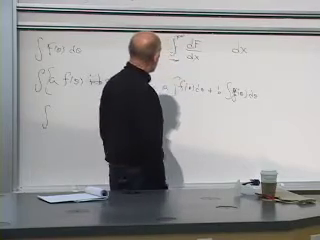
\includegraphics[width=0.88\textwidth]{lecture_06_figure_05.png}\lectureframe{01:26:31.594}\caption{Modèle ordinaire de l’intégration de Berezin : l’intégrale d’une dérivée totale se réduit aux valeurs aux bornes et s’annule lorsque la fonction tend vers zéro à l’infini. La ligne inférieure du tableau est en partie masquée ; l’équation est donc reproduite clairement dans le texte.}\end{figure}

Nous voulons que l’intégrale de Grassmann soit linéaire et possède la propriété utile selon laquelle l’intégrale d’une dérivée totale est nulle. Pour une coordonnée impaire, imposons
\begin{align}
\int d\theta\,[af(\theta)+bg(\theta)]
&=
a\int d\theta\,f(\theta)
+b\int d\theta\,g(\theta),\\
\int d\theta\,\partial_\theta f(\theta)&=0.
\end{align}
La seconde condition est l’analogue algébrique de l’invariance par translation de la mesure. Il n’y a ni bornes sur une droite des nombres impairs ni somme sur de petits intervalles.

\begin{classroomqa}\audiencequestion{S’il n’existe pas d’intégrale indéfinie de Grassmann, renonce-t-on à l’idée que l’intégration est l’opération inverse de la dérivation ? \lecturetimestamp{01:21:19}}\lecturerresponse{Oui. L’intégration de Berezin est une forme linéaire définie, et non une opération de recherche de primitive. Pour une variable de Grassmann, elle est en fait représentée par la même opération algébrique que la dérivation.}\end{classroomqa}

\begin{classroomqa}\audiencequestion{L’intégration sur tout l’espace-temps, \(d^4x\), est-elle elle aussi une intégrale définie ? \lecturetimestamp{01:21:34}}\lecturerresponse{Oui. Les conditions aux limites sont sous-entendues lorsqu’on intègre l’action sur l’espace-temps. La différence est que l’intégration ordinaire sur l’espace-temps peut se comprendre comme une limite de sommes, tandis que l’intégration de Grassmann est définie algébriquement par son action sur la base finie \(1,\theta\).}\end{classroomqa}

\subsection{Une variable}

Toute fonction d’une variable impaire peut s’écrire en plaçant son coefficient dans l’ordre fixé, à droite :
\begin{equation}
f(\theta)=a+\theta b.
\end{equation}
Comme \(\partial_\theta\theta=1\), la règle de dérivée totale implique
\begin{equation}
\int d\theta\,1=0.
\end{equation}
On choisit la normalisation restante de sorte que
\begin{equation}
\int d\theta\,\theta=1.
\end{equation}
Par conséquent,
\begin{equation}
\int d\theta\,f(\theta)=b.
\end{equation}
L’intégrale extrait le coefficient de la plus grande puissance possible. Avec la convention de dérivation à gauche utilisée ici,
\begin{equation}
\partial_\theta f=b
=\int d\theta\,f.
\end{equation}

\begin{classroomqa}\audiencequestion{Existe-t-il une fonction \(F(\theta)\) telle que \(\partial_\theta F=\theta\) ? \lecturetimestamp{01:30:05}}\lecturerresponse{Non. Une telle fonction devrait comporter un terme proportionnel à \(\theta^2\), mais \(\theta^2=0\). C’est une autre façon de voir pourquoi il n’existe pas d’analogue de la primitive indéfinie pour les variables de Grassmann.}\end{classroomqa}

\subsection{Deux variables et l’ordre de la mesure}

Pour une paire complexe \(\theta,\bar\theta\), écrivons une fonction paire générale sous la forme ordonnée
\begin{equation}
f(\theta,\bar\theta)
=a+\bar\theta\psi+\bar\psi\theta+b\,\bar\theta\theta.
\end{equation}
Il n’existe pas de terme d’ordre supérieur, car
\begin{equation}
\theta^2=\bar\theta^2=0,
\qquad
\bar\theta\theta=-\theta\bar\theta.
\end{equation}

Fixons maintenant la convention
\begin{equation}
\int d\theta\,d\bar\theta\,
\bar\theta\theta=1.
\end{equation}
Dans les intégrales itérées, l’opération \(d\bar\theta\) adjacente agit en premier. On obtient alors le tableau suivant :
\begin{align}
\int d\theta\,d\bar\theta\,1&=0,\\
\int d\theta\,d\bar\theta\,\theta&=0,\\
\int d\theta\,d\bar\theta\,\bar\theta&=0,\\
\int d\theta\,d\bar\theta\,\bar\theta\theta&=1.
\end{align}
Ainsi,
\begin{equation}
\int d\theta\,d\bar\theta\,
f(\theta,\bar\theta)=b.
\end{equation}

\begin{classroomqa}\audiencequestion{Pour un terme linéaire en \(\theta\), est-ce bien l’intégration par rapport à \(\theta\) qui rend l’intégrale double nulle ? \lecturetimestamp{01:34:59}}\lecturerresponse{Non ; l’explication donnée oralement inversait les rôles. L’intégration par rapport à \(\theta\) de \(\theta\) donne un. Le résultat ne contient alors plus de \(\bar\theta\), et l’intégrale restante de un par rapport à \(\bar\theta\) s’annule. Dans tous les cas, l’intégrale double n’est non nulle que si les deux variables sont présentes.}\end{classroomqa}

\begin{classroomqa}\audiencequestion{Si l’on intervertit \(\theta\) et \(\bar\theta\), l’intégrale change-t-elle de signe ? \lecturetimestamp{01:36:33}}\lecturerresponse{Oui. Les variables impaires et les mesures impaires anticommutent. Avec la convention ci-dessus,
\[
\int d\bar\theta\,d\theta\,\bar\theta\theta=-1.
\]
Il faut donc choisir un ordre et le respecter systématiquement. La physique est indépendante de la convention, mais les signes intermédiaires ne le sont pas.}\end{classroomqa}

Pour \(n\) variables de Grassmann indépendantes, la règle est immédiate :
\begin{equation}
\int d\theta_n\cdots d\theta_1\,
f(\theta_1,\ldots,\theta_n)
\end{equation}
extrait le coefficient du monôme ordonné de plus haut degré
\(\theta_1\cdots\theta_n\), au signe près, lequel est fixé par l’ordre choisi pour les variables et les mesures. Cette simple règle d’extraction des composantes est au cœur des actions en espace supersymétrique. Une variation supersymétrique devient une dérivée totale impaire, que l’intégrale sur l’espace supersymétrique élimine, tout comme une action ordinaire élimine une dérivée totale dans l’espace-temps lorsque les conditions aux limites le permettent.

\section{Pourquoi un calcul si élémentaire a-t-il autant de puissance}

Les règles semblent presque triviales :
\begin{equation}
\int d\theta\,1=0,
\qquad
\int d\theta\,\theta=1.
\end{equation}
Pourtant, elles nous permettent de construire des théories des champs avec interactions dans lesquelles les relations entre masses et constantes de couplage bosoniques et fermioniques sont automatiquement préservées. Le calcul en espace supersymétrique a le même objectif que le calcul tensoriel en relativité : organiser la notation de façon que la symétrie recherchée soit préservée par toutes les manipulations autorisées.

La gestion des signes en est le prix. Chaque permutation de deux objets impairs introduit un signe moins, et un calcul peut être juste sur le plan conceptuel tout en comportant une erreur due à un seul choix d’ordre. Cette difficulté n’est pas accessoire ; elle est le reflet algébrique de la statistique fermionique.

\begin{classroomqa}\audiencequestion{Les nombres de Grassmann ont-ils été inventés en même temps que la supersymétrie, ou existaient-ils déjà ? \lecturetimestamp{01:41:19}}\lecturerresponse{Ils sont bien plus anciens. Hermann Grassmann a développé l’algèbre extérieure sous-jacente au dix-neuvième siècle. Les formes différentielles utilisent déjà des éléments de base anticommutants ; la théorie quantique des champs et la supersymétrie du vingtième siècle ont donné un nouveau rôle physique à ces mêmes mathématiques.}\end{classroomqa}

Nous sommes maintenant prêts à passer à des constructions concrètes. Les superchamps regroupent des multiplets boson-fermion complets, les dérivées dans l’espace supersymétrique préservent l’algèbre, et l’intégration de Berezin extrait l’action en composantes. L’étape suivante consiste à utiliser cet outillage dans le modèle le plus simple à une dimension, puis à le transposer à la théorie des champs.
